\documentclass[]{Photos_interface_design}
\usepackage{graphicx}
\usepackage{hyperref}
\usepackage{eurosym}
\usepackage{pifont}
%\usepackage{tocloft}
\usepackage{amsmath}
\usepackage{subfigure}

\makeatletter
\renewcommand*\l@subsection{\@dottedtocline{2}{1.5em}{2.0em}}
\renewcommand*\l@subsubsection{\@dottedtocline{3}{3.0em}{3.0em}}
\makeatother

\begin{document}

\maketitle

\tableofcontents\pdfbookmark[0]{Table of Contents}{toc}

\newpage

\section{Introduction}
Since long, {\tt PHOTOS} Monte Carlo \cite{Barberio:1990ms,Barberio:1993qi} is used for generation for bremmstrahlung in decay of particle and resonances. Over the years program acquired
popularity and discussion of its systematic error, was pushed to high 
precision \cite{Golonka:2006tw}. Multiphoton radiation was introduced \cite{Golonka:2005pn} phase space treatment was shown to be exact \cite{Nanava:2006vv} and for several processes \cite{Golonka:2006tw,Nanava:2006vv,Nanava:2009vg}
exact matrix element was introduced with the help of optional weights.
Benchmarks distributions including comparisons with  
other simulation programs were collected on program web page \cite{Photos_tests}. 

 Such high precision applications require good control of the event record content on which {\tt PHOTOS} operates. On one side it 
requests skills and experience of the user on the other it provides 
flexibility necessary for study of effects like systematic errors for 
measurements of anomalous couplings or W mass for example. Methods of 
correlated samples  can be applied\footnote{To exploit such methods in 
high precision regime, good control of matrix element properties is necessary
\cite{Kleiss:1990jv}} 

Until recently {\tt HEPEVT} was used as structure for 
communication between physics Monte Carlo programs and Detector/reconstruction 
packages. Experimental physicists were using that structure 
for their own applications  as well.

Recently, to gain  flexibility {\tt FORTRAN} is  replaced by C++ and 
instead of {\tt HEPEVT}, the C++ event structure called {\tt HepMC} \cite{Dobbs:2001ck}
is used. Nothing prevents 
moving {\tt PHOTOS} to environment based on  {\tt HepMC}
 and rewrite whole (at first event record dependent parts) 
of {\tt PHOTOS}\footnote{Up to date version of the code described in this paper is
available from web page of our project~\cite{photosC++}. 
As we are still in the phase of refining
we change the program (and update this note) on regular basis. 
This can be a problem if bug fixing is necessary and user has invested time 
in temporary version. To overcome this difficulty, 
together with the code, information of the code version registered in 
SVN server is available.  }
 to C++. In fact implementation of the algorithm is clearer and easier to
 maintain. Because of its design {\tt PHOTOS} algorithm benefit from object 
oriented features of C++. It is our third program, after {\tt MC-TESTER} \cite{Davidson:2008ma}
and {\tt TAUOLA} interface \cite{Davidson:2010rw} which is ported to {\tt HepMC} and C++.
This completes main step of migration of these 3 programs to new style.

Such migration is convenient for the users too,  they can now work
with  homogenous C++ software. From physics point of view transformation 
of {\tt PHOTOS} 
from {\tt FORTRAN} to C++  bring some benefits as well.
Channel dependent matrix elements of {\tt PHOTOS}, in {\tt FORTRAN} available only 
in special, process dependent versions and working for some special
kinematical configurations
can be now installed for general use.
For that purpose, better access to information available in event records
will be provided already now.



Our paper is organized as follows ...



\section{Requirements of the {\tt PHOTOS} Interface}
The algorithm of {\tt PHOTOS} Monte Carlo can be divided into two parts.
Internal one, operates on elementary decays. Thanks to carefully 
studied properties of 
QED (scalar QED) algorithm, with certain probability, 
replace  kinematical configuration of Born level decay by a new one, 
where bremsstrahlung photon or photons
may be present. This part of the program is sophisticated from the physics 
point of view \cite{Nanava:2006vv,Golonka:2006tw},
but from the point of view of data structure algorithms is simple.
That is why, gain from re-writing this part of the program to C++ is rather
limited and will be postponed at this step of the project development.
On the other hand, there are no much obstacles for such transformation to 
perform. In fact such transformation was performed already
previously \cite{photosplus}, but resulting program was developed too early 
and did not attracted users.

Typical result of high energy process simulation are events of complex structure:
they include, for example initial state parton showers, hard scattering parts 
hadronization and finally chains of cascade decays of resonances. 
Structure similar to a tree is created, but properties of such data structure
tree are sometimes violated.
For its action {\tt PHOTOS} need to scan event record (tree) 
and localize branchings where
it is supposed to act. Decaying particle (mother) and its primary decay products
daughters have to be passed into internal event structure of {\tt PHOTOS}. 
Finally for each daughter list of all its subsequent decay products has to be 
formed. It is needed as kinematical modification need to be performed on each 
member of those list accordingly to change introduced to primary daughter.

In new C++ version of this part of the algorithm additional functionality
is provided.
First mother of the decaying particle will be localized and supplement 
elementary branching. 

Prior to activation
of the {\tt FORTRAN} part of the algorithm all decay branching 
(supplemented with the first 
mother) will be boosted to decaying particle rest frame and first mother
will be oriented along z axis.

We can summarize that the following operations must be implemented
in our event record interface:
\begin{enumerate}
\item method to search for elementary decays over all tree of the event
\item method to form lists of all subsequent decay products originating from each elementary decay products.
\item method to localize first mother of decaying particle 
\item method to localize second mother of $t \bar t$ pair.
\item method to read  particles stored in the event tree.
\item method to add or modify particles of the event tree.
\end{enumerate}

TXT\footnote{ {\bf remnant text}  

{\tt PHOTOS} act on such vertex and modifies four momenta of residing there daughters 
and eventually adds new ones that is photons. 
Such procedure is exact from the point of view of phase space; for details see eg.  approximation in on flight constructed matrix elements are based
on factorization properties of QED. 

In case one is interested to go beyond that precision level, one has to  provide
more information. Spin state of the decaying particle has to be passed to the code calculating matrix element. For that it is enough to store into event record
information on particles or fields resulting in creation of
our particle under consideration that is mother for the decay vertex.
It is then convenient to transform all particles to the rest frame of the Mother
and orient Mothers mother along z axis before passing the information from HepMC to {\tt PHOTOS} internal data structure. Let us call resulting Lorentz transformation $L$. Once PHOTOS internal algorithm complete
its action all four momenta have to be transformed back by $L^{-1}$ and 
modification of remaining part of the event record (replacement of momenta
add of new photons to HepMC and modification of all descendants of 
daughters would be performed as in more standard case explained above.
}

\subsection{C++ Specific Requirements}

The C++ version of the {\tt PHOTOS} interface implements all functionalities
of its predecessor, the {\tt PHOTOS} coded in {\tt FORTRAN}.
It can be attached to any Monte-Carlo program,
provided its output is available through a {\tt HepMC} \cite{Dobbs:2001ck} event record.

This condition is not very restrictive, is seems that {\tt HepMC} will
remain a generally accepted standard for the near future. However,
already now several different options for how {\tt HepMC} is used are
widespread. Possibility of the flexible  adaptation of our event record 
interface to different
options has been considered in the design,  drawing experience
from {\tt MC-TESTER} \cite{Golonka:2002rz,Davidson:2008ma}.
We have also
envisaged the possibility that {\tt HepMC} may one day be replaced by another
standard of event record, and we have provided an easy way to extend
the interface to a possible new event record standard.

\subsection{Object Oriented Event Records  -- The Case of {\tt HepMC}}
In adopting {\tt PHOTOS} interface to the C++ event record format
 the difference between the {\tt HEPEVT} event record used in the {\tt FORTRAN}
version of {\tt PHOTOS} interface and {\tt HepMC} event record  
which is used for the C++ based interface
has to be taken into account. 
In the first case the whole event was represented
by a common block containing a list of particles with their properties and
with integer 
variables denoting pointers to their origins and descendants.
 The {\tt HepMC} event structure
is built from vertices, each of them having pointers to their origins and descendants. Links between vertices represent particles or fields.
 In both, {\tt FORTRAN} and C++  
cases, the event is structured as 
a tree\footnote{At least in principle, because in practice its properties
may be rather of the graph of not universally defined properties.
This makes our task challenging.}, the necessary algorithms are  analogous, 
but nonetheless different. The {\tt HepMC} structure based on vertices is more
convenient for {\tt PHOTOS} interface

In {\tt HepMC version 2.04}, an  event is represented by a {\tt GenEvent} object,
which contains all information regarding itself, including event id,
units used for dimensional quantities in the event and the list of produced particles. The particles
themselves are grouped into {\tt GenVertex} objects allowing access to mother
and daughter particles of a single decay. Vertices provide an easy way
to point to the whole branch in a decay tree that needs to be accessed,
modified or deleted if needed. The information of a particle  itself is stored
in a {\tt GenParticle} object containing the particle id, status and momentum
as well as information needed to locate its position in the decay tree.
This approach allows traversing the event record structure in several different
ways.

The {\tt HepMC} event record format is  evolving with time, making it necessary
 to adapt
the code to the new versions.
{\tt HepMC} version 2.05 is used as a reference. In the case of version 2.03 restrictions on methods for 
units
conversion have to be taken into account, for details see Appendix B.5
of ref. \cite{Davidson:2010rw}. At present we have not yet introduced such 
backward compatibility downgrade for {\tt PHOTOS}. It is probably not necessary.
However,
one should keep in mind that future adaptations to {\tt HepMC} changes may restrain
backward compatibility.

Evolution of the {\tt HepMC} format itself is not a crucial problem.
In contrary, conventions how physics information is  filled into {\tt HepMC}
 represent the source of main technical and also physics 
challenge for our interface. 
This is quite similar to the previous
{\tt HEPEVT - FORTRAN} case. Let us discuss this point in more detail now.

\subsubsection{Event Record Structure Scenarios}

{\bf PYTHIA,HERWIG,MC@NLO etc. }

While many Monte-Carlo generators (eg.. {\tt PYTHIA 8.1} \cite{Sjostrand:2007gs}, 
HERWIG++ \cite{Bahr:2008pv})
store events in {\tt HepMC} format, the  representations of
these events are not subject to strict standards,  which can therefore
vary between Monte-Carlo generators or even physics processes. Some examples
of these variations include the conventions of status codes, the  way
documentary information on the event is added, the direction of pointers at a vertex
and the conservation (or lack of conservation) of energy-momentum at a vertex.
Below is a list of properties for basic scenario we have observed in Monte-Carlo
generators used for testing the code.

This list will serve as a declaration for convention of  {\tt HepMC} filling, which  the 
interface should  be able to interpret correctly.

\begin{itemize}
  \item \textbf{4-momentum conservation} is assumed for all vertices in the event record where {\tt PHOTOS} is expected to act.
  \item \textbf{Status codes:} only information whether given particle is incoming, outgoing or intermediate will be used,
  \item \textbf{Pointers at a vertex} are assumed to be bi-directional. That is, it is possible to traverse the record structure from mother to daughter and from daughter to mother along the same path.
\end{itemize}

\noindent
\textbf{ Extensions/Exceptions} to this specifications  are handled in some cases. We will call them
options for conventions of event record filling.
  \begin{itemize} 
    \item  Vertices like $\tau^\pm \rightarrow \tau^\pm$ and $\tau^\mp \rightarrow \tau^\mp \gamma$ 
           where 4-momentum conservation is not preserved. Due to 4-momentum non-conservation,
           {\tt PHOTOS} will not be invoked.
    \item
           As in the {\tt FORTRAN} cases, we expect that  new  types of 
           conventions for filling the event record
           will appear, because of physics motivated requirements.
           Unfortunately, the resulting options do not always guarantee
           an algebraically closed structure.  
           Host program specific patches  may need to be defined for the 
           {\tt TAUOLA interface}. 
           Debugging it could be time consuming, and will need to be repeated for every new
           case.
   \end{itemize}


Detailed
conventions for the actual filling of physics information into {\tt HepMC} format
is defined by authors of each Monte Carlo program.
 In future,  an important special case of event records filling with
information extracted from experimentally observed event (eg. $Z\to \mu^+\mu^-$
 modified later to $Z\to \tau^+\tau^-$) should be allowed.
  Obviously, a new type (or types) of {\tt HepMC} filling will then appear.

Good example is evolution of {\tt PYTHIA}. While in version 8.108 status codes for 
our example processes were  taking values 0, 1, or 2  in part of the record 
important for {\tt PHOTOS} functioning, changes were already present in
 version 8.135. As consequence status code for 
otherwise nicely decaying particles was not anymore 2. We have introduced 
patch for that in file PhotosEvent.cxx. After patch 
program should work with older version as well, but we are not sure if there 
are no negative consequences. Tests are on going. We are also investigating 
if instead of patches new input of {\tt PYTHIA} would not be more appropriate 
solution for us.

We need to make our mind on bar codes conventions. Our programs, {\tt TAUOLA} and
 {\tt PHOTOS} supplement event record with new particle entries carrying bar codes 
increased by 10000 with respect to the value which would be given if such 
particles were generated by main generator. It is not clear to us if it is 
reasonable choice from the point of view of program users.

\subsection{Interface to event record of {\tt FORTRAN}}
\label{sect:F77fill}
In principle it would be rather simple to re-write whole {\tt PHOTOS} into
C++. However to profit from the numerical tests, for the time being its part
is still left in {\tt FORTRAN}. The C++ part of the code search the whole event for
suitable for generation of bremsstrahlung vertices in HepMC. Once such
vertex is found it is copied to internal event record  which is 
called  {\tt PH$\_$HEPEVT} (this is effectively a copy of {\tt HEPEVT};
 event record of {\tt FORTRAN}.
and then {\tt FORTRAN} code of {\tt PHOTOS} is executed.
The data structure passed this way is rather simple. Single vertex
supplemented with mothers of decaying particle are passed only. Information 
on mothers will be useful in future for calculation of process dependent 
kernels. Another data structure of   {\tt HEPEVT} type {\tt PHOEVT} is also 
used in {\tt PHOTOS}. It is used to store the decay vertex only. Obviously 
the two structures are of the temporary need and should disappear rather soon.

For details on interface to {\tt FORTRAN} see appendix \ref{Interface to PHOTOS}.


\section{Design}

\subsection{Classes and Responsibilities}

The choice of splitting the source code into three main modules
allows to separate the {\tt FORTRAN} related code from the abstract C++ interface
and the concrete implementation of the interface created for the appropriate
event record.

\begin{figure}[h!]
\centering
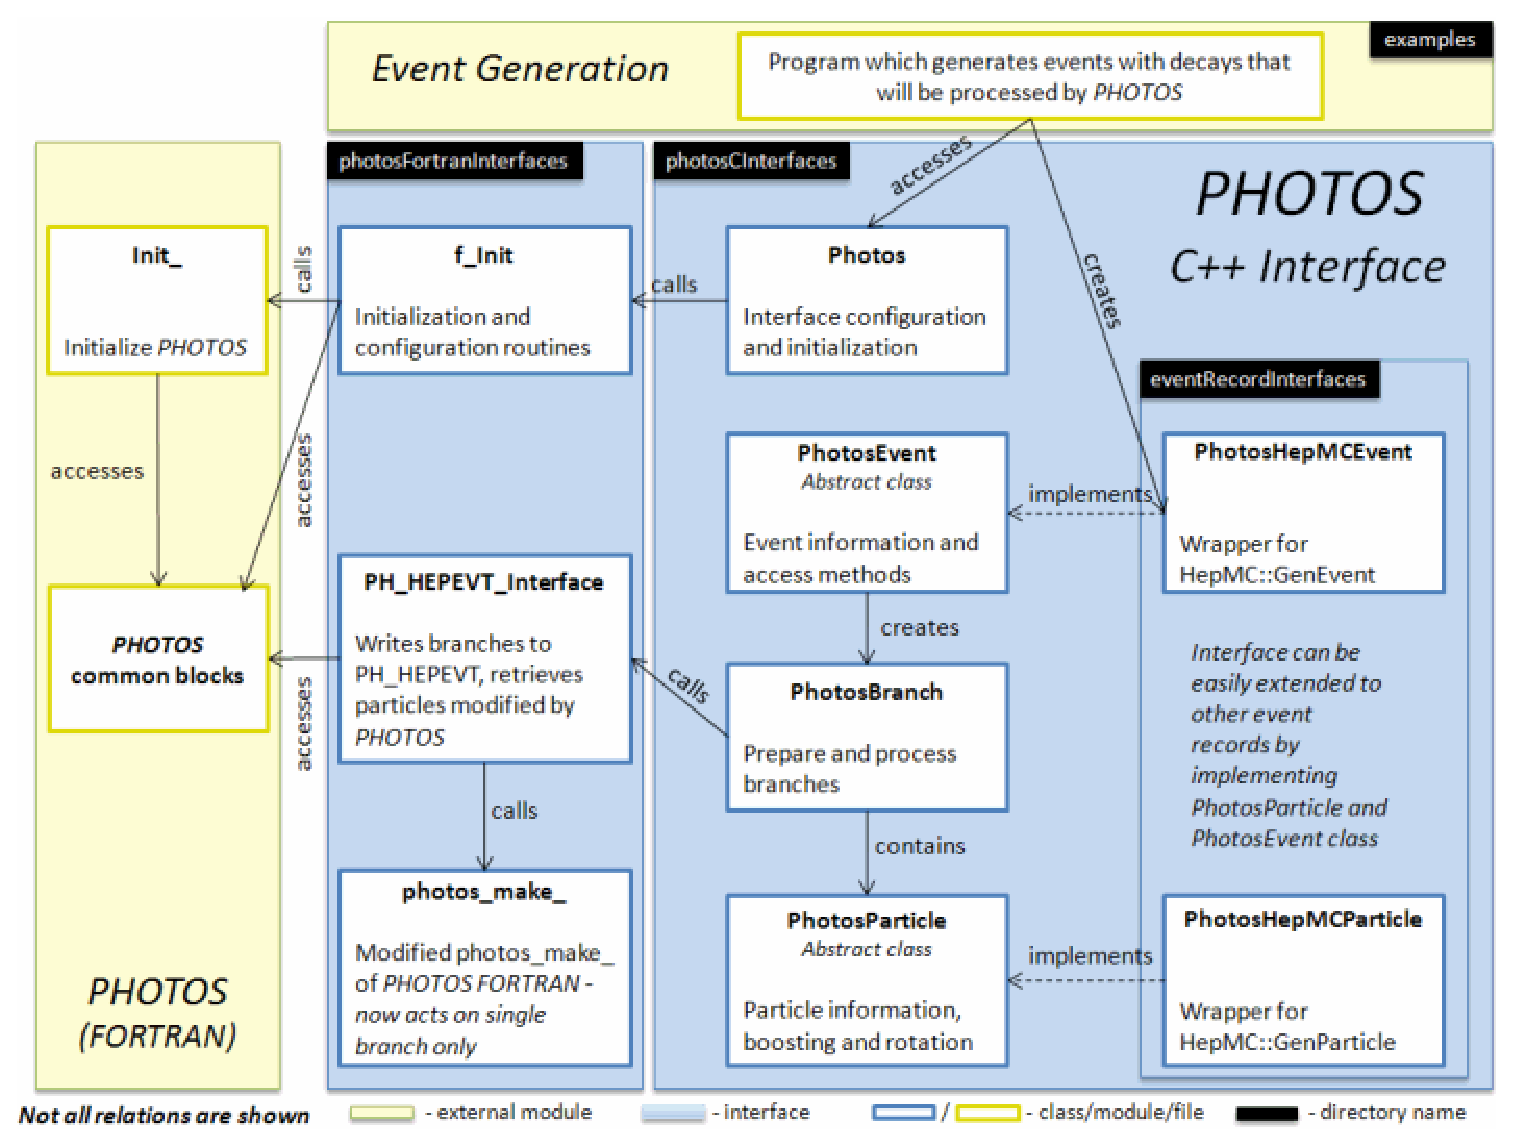
\includegraphics[scale=0.6]{interface_design.eps}
\label{fig:design}
\caption{{\tt PHOTOS} C++ interface class relation diagram}
\end{figure}

\begin{itemize}
  \item {\bf {\tt PHOTOS FORTRAN} Interface}\\
       This part of the code provides an interface 
       to the {\tt FORTRAN} library of {\tt PHOTOS}. In particular,  routines
       necessary for library initialization and wrapper for routine invoking the processing
	   of single branch. Parts of the interface code are still left in {\tt FORTRAN}, but
	   can be rather easily rewritten to C++. 
       The most important part, {\tt PH\_HEPEVT\_Interface\_},
       is already implemented  in C++. This method is responsible for writing
	   decay branch that needs to be processed to HEPEVT.
       For further details see Appendix \ref{Interface to PHOTOS}.
  \item {\bf {\tt PHOTOS} C++ Interface} \\
       The abstract part of the interface to the event record.
       The class {\tt PhotosEvent} contains information regarding the whole event
       structure, while {\tt PhotosParticle} stores all information regarding a single particle.
       All particles used by the interface are located in the event in the form of
       a list of {\tt PhotosParticle} objects.
       The last class located here, {\tt PhotosBranch}, contains information regarding
	   single branch to be processed by {\tt PHOTOS}.
  \item {\bf Event Record Interface} \\
       The event record implementation classes. All classes stored here represent
       the implementation of specific event record interfaces and are responsible for reading,
       traversing and writing to the event record structure.
       Only {\tt PhotosEvent} and {\tt PhotosParticle} classes must be implemented.
       The {\tt HepMC} event record interface is implemented
       through {\tt PhotosHepMCEvent} and {\tt PhotosHepMCParticle}.
\end{itemize}

\subsection{Directory Structure}

\begin{itemize}
\item {\bf src/eventRecordInterfaces/ } - source code for classes which interface with {\tt HepMC}.\\
  Classes:
  \begin{itemize}S
  \item { \bf PhotosHepMCEvent} - Interface to HepMC::GenEvent objects. 
  \item { \bf PhotosHepMCParticle} - Interface to HepMC::GenParticle objects. 
  \end{itemize}   

\item {\bf src/photosCInterfaces/ } - source code for general {\tt PHOTOS} interface.  \\
  Classes:
  \begin{itemize}
  \item { \bf Photos } - Controls the configuration and initialization of {\tt PHOTOS FORTRAN}.
  \item { \bf PhotosEvent } - Abstract base class for event information.
  \item { \bf PhotosParticle } - Abstract base class for particles in the event.
  \item { \bf PhotosBranch } - Contains one {\tt PhotosParticle} object, its mothers and daughters.
  Filtering branches sent to {\tt PHOTOS} is done here.
  \end{itemize}

\item {\bf src/photosFortranInterfaces/ } -  interface to {\tt PHOTOS FORTRAN} routines and common blocks. \\
  Files:
    \begin{itemize}
    \item { \bf f\_Init } - contains a wrapper for the {\tt PHOTOS FORTRAN} routines for initialization.
    \item { \bf PH\_HEPEVT\_interface } - contains wrapper for accessing HEPEVT common block.
    \item { \bf photos\_make.f } - contains extra {\tt FORTRAN} routines which should ultimately be migrated to C++.
    \end{itemize}

\item {\bf src/utilities/ } - source code for utilities that help debugging.\\
  Classes:
  \begin{itemize}
  \item { \bf Log} - General purpose logging class that allows filtering out output messages 
      of {\tt PHOTOS C++ Interface} and keeps statistics regarding each run.
  \end{itemize}   

  \item {\bf examples/ } - examples of different {\tt PHOTOS} C++ Interface uses
    \begin{itemize}
	\item {\bf photos\_standalone\_example} - the most basic example which loads pre-generated 
	      events stored in file in {\tt HepMC} format which are then processed by {\tt PHOTOS}.
	\item {\bf single\_photos\_gun\_example} - an example of using the {\tt processOne} method
	      to process only selected particles within the event record.
    \item {\bf photos\_pythia\_example} - simple $e^+e^- \rightarrow Z \rightarrow e^+e^-$ event in
	{\tt HepMC} format which is then processed by {\tt PHOTOS}.
    \item {\bf tauola\_photos\_pythia\_example } - example of  {\tt TAUOLA} linked with {\tt PYTHIA 8.1},
	and decay chain processed by {\tt PHOTOS} and analysed with  {\tt MC-TESTER}.
    \end{itemize}   
  \item {\bf include/} - directory for the header files.
  \item {\bf lib/ } - directory for the compiled  libraries. 
  \item {\bf documentation/ } - contains doxygen documentation and this latex file.
  \item {\bf photos-fortran/ } standard {\tt PHOTOS FORTRAN} distribution
\end{itemize}

\subsection{Algorithm Outline}
\label{sect:Outline}

An overview of the algorithm for  the {\tt PHOTOS C++ Interface} is
given below. For clarity, the example assumes that the processed event
is stored in {\tt HepMC} event record structure.

The first step is creation of a {\tt PhotosHepMCEvent} object from
a {\tt HepMC::GenEvent} event record. After that, the {\tt process()} method should
be executed by the user's code\footnote{Prior to this step
the user may want to execute {\tt Photos::processParticle(...)} or {\tt Photos::processBranch(...)}
for branches, where {\tt PHOTOS} is expected not to work properly or if only one branch
needs to be examined by {\tt PHOTOS}. For details see Appendix~\ref{PHOTOSgun}.
}, invoking the following process:

\begin{enumerate}
\item The {\tt HepMC} event record is traversed and a list of all decaying
      particles is created.
\item Each particle is checked and if it's a self-decay, the particle is filtered out.
\item From the remaining particle, a branch containing particles mothers and daughters
      is created. Special cases with no intermediate particle are handled and the
	  list of branches is created.
\item Branches are filtered out depending on the user choices of processes
      that need to be skipped by {\tt PHOTOS}.
\item Now, each branch is processed by {\tt PHOTOS} separately:

	\begin{enumerate}
  
	\item The branch is written to HEPEVT
	\item {\tt PHOTOS} is invoked with the index of particle from which the branch
	      has been created
	\item The resulting branch is taken back from HEPEVT integrating any changes
	      made by {\tt PHOTOS}. New particles are created and the old ones are modified
		  accordingly.

	\end{enumerate}

\end{enumerate}

The underlying HepMC::GenEvent is hence modified with insertion of photons.

\section{Extensibility}
 The purpose of the present version of C++ interface to {\tt PHOTOS} is to enable 
all functionality of its {\tt FORTRAN} predecessor to be available for HepMC data
structure. Some methods for better initializations are already introduced
now. Some arrangements were introduced to enable further
extensions in future. Let us briefly discuss some of these points.
 
\subsection{{\tt PHOTOS} Extensions}
In the present paper we have presented an algorithm as of today. 
That is the version which is compatible with the one implemented in {\tt FORTRAN}.
As it can be seen from the text of presentation we have prepared the structure 
for implementation of channel dependent matrix elements. This work, scattered
 over special corrections to the {\tt FORTRAN} version applicable one at a time can  
be simply integrated all together into C++ version.
 At present we are however not convinced if such complication is worth 
the complication for the user as it request more strict control of event 
record content and gain of precision, which is quite good already now is 
not that important. That is why, we have not completed migration to C++.
Instead as intermediate step we complete work on tests, prior to re-write
 of numerically sensitive part which at the same time is algorithm-wise rather 
simple.
Methods deviced to check content of HepMC as used by {\tt PHOTOS} were already 
described in Appendix \ref{App:Logging}. They need to be used whenever {\tt PHOTOS} 
is expected to work with new source of event record fills originating eg. 
from upgrades of  {\tt PYTHIA}. 
Over the years of work with the algorithm it turned out that this is the
most demanding work, 
necessity to adopt to varying physics and technical input of event record
pose a multitude of problems. Nature of difficulties can not be predicted 
in advance.


For the sake of debugging we have introduced control methods to activate
 internal printouts of {\tt FORTRAN} part of the code.
Routine PHLUPA \cite{Barberio:1993qi} is activated and one can verify  
for the event offending for example  energy momentum conservation how it is 
constructed. That is quite convenient for tracing inconsistencies in 
information passed to {\tt PHOTOS} for example. 


Numerical stability is another  problem. It can not be separated from
 physics constraints. Condition  $E^2-p^2=m^2$ may be broken  because of 
rounding errors. However in the same event but for other particle, this on 
mass shell 
condition may not be correct as some intermediate particles present in event 
records may have substantial widths. 
{\tt PHOTOS} may become adaptable to such varying conditions, but it requires
good interaction with the users. Protection against some reversible
inconsistencies in event record may be the source of unexpected difficulties
for other cases. At present this is left to {\tt FORTRAN} part of the algorithm.
This will gradually migrate to C++


 
\subsection{Event Record Interface}
In {\tt FORTRAN} times {\tt PHOTOS} interface was using structure which was effectively
inheriting from  HEPEVT
adding to it (understood as a data type) extra variable defining 
status of particles with respect to QED Bremsstrahlung. In some cases like
$\tau \to l \nu_l \nu_\tau$ bremsstrahlung was already generated earlier
and if {\tt PHOTOS} would act on it then double counting would arise.
At present, instead of such arrangement set of initialization methods is 
prepared and described in section \ref{section:suppress}. There is a definite room for 
improvement. For example if vertex $q \bar q \to l^\pm l^\mp g$ is encountered,
interface can `on flight' add intermediate $Z$ to the record and enable {\tt PHOTOS}
on such temporarily constructed decay branching $Z \to l^\pm l^\mp $.


 Internally in {\tt FORTRAN} part of {\tt PHOTOS}
data structure of HEPEVT type PH\_HEPEVT and PHOEVT are used, but  to store 
single elementary decay only. At this step in program evolution it is may be 
not the most elegant solution, but leaves lot of {\tt FORTRAN} time benchmarks 
with no  need to redo.




\section{Testing}

One of the most important part of {\tt PHOTOS} project are its physics oriented tests.
Several domain
of physics tests should be mentioned. For user interested in precision 
simulation of Z or W decay the most interesting will be papers \cite{Nanava:2009vg,Golonka:2006tw}. There, careful comparison with first order matrix element 
and confirmation that algorithm scheme  is compatible with exclusive 
exponentiation was the prime target. Compatibility of the solution
with second order matrix element are less important. 
It is important to know that missing in first order EEX or CEEX \cite{koralz4:1994,kkcpc:1999} 
scheme terms
lead to effects which are typically of the order of 0.2 \% but are at the level 
or 30 \% or more in double hard photon region of the phase space. That is 
why it may lead to effects which are more important when complex experimental 
cuts are applied\footnote{We thank Andy Buckley for checking numerically
 that such limitation is present in many presently used monte Carlo programs,
in particular Sherpa and Herwig++.  } 
for the measurements of $W$'s or $Z$'s.
 For users interested in simulation of
bacground for Higgs searches at LHC and for any other applications where 
two hard photon configurations are important studies based on comparison with 
double photon matrix element are of 
interest \cite{Barberio:1993qi,RichterWas:1994ep,RichterWas:1993ta}.
Finally user interested in low energy processes where underlying physics model 
for photon emission can not be controlled in full by theory; scalar QED may 
be considered only as the starting point will profit 
from \cite{Nanava:2009vg,Nanava:2006vv}. In all cases it is important that
 program generation cover the full phase space and that there are no 
approximation in its treatment. In contrary, as in {\tt FORTRAN} version code 
features approximation in the kernel. In some cases process dependent 
complete first order 
kernel is available but is not installed in public version  
because resulting approximation is 
numerically unimportant and requires control of the spin state for decaying 
particle. That requires better control of event record than what was available 
in {\tt FORTRAN}. At present such option is prepared see section \ref{sect:F77fill} but not exploited. 

The main purpose of the present paper is program documentation. That is why
we concentrate on program tests required to guarrant its proper installation.
Discussed above physics tests
do not guarranty that the program will perform well on a particular platform and installation. Tests and debugging
is necessary.  If content of the event record is non-standard or rounding error are large {\tt PHOTOS} performance will deteriorate.

The first check of {\tt PHOTOS} installation is if some energy momentum non 
conservation would appear. Such offending events should be looked at
before {\tt PHOTOS} action and after.
If impossible to understand why inconsistencies for energy momentum non 
conservation are created by {\tt PHOTOS}, authors should be contacted. Sometimes
monitoring of how event is constructed inside {\tt FORTRAN} part of the code
may be useful. For that purpose its steering parameters .... are
available form C++ part of the code. In practice only rather
 advanced user will have possibility to understand the printouts. They may be 
useful for authors to understand the cause of the trouble.

The next step in benchmarking rely on comparison with benchmark distributions. 
At present we store them with the help of ROOT system and our {\tt MC-TESTER} tool



\subsection{Benchmarks with {\tt MC-TESTER}}
Over the years of development of {\tt TAUOLA} and {\tt PHOTOS} programs certain level 
of automatization of tests was achieved. It was found that monitoring all invariant masses which can be constructed out from a given decay represent 
quite restrictive and still easy to implement test. We have applied such method 
for {\tt PHOTOS} too. In this case however some soft, final state particles have to be ignored. Finding of relative fractions of events with distinct final states 
was complementing that test implemented now in public version of {\tt MC-TESTER}
working with infrared unstable samples too. See section .... of 
ref \cite{Davidson:2008ma} for more details. For standard decay modes benchmarks are collected on our project web page \cite{Photos_tests}.
Here we have collected numerical results in directory 
{\tt examples/testing} and its subdirectories; respectively  
{\tt Htautau, ttbar, Wenu, Wmunu, Zee, Zmumu}. Each of those include
appropriate initialization files for the particular run of {\tt PYTHIA}. Numerical results from long runs of {\tt MC-TESTER} based tests
are stored for reference. Our choice of tests, at present is oriented toward 
LHC user and radiative corrections in decay of W's, Z's and Higgs particles.
At present users of low energy experiments are often using {\tt FORTRAN} version 
of the code. 


\subsection{Results}
\label{sec:results}
In principle, at the level of single splitting the C++ interface of {\tt PHOTOS}
introduces nothing new with respect to standard version of {\tt PHOTOS} as available 
in {\tt FORTRAN}. That is why, standard tests as collected in \cite{Photos_tests} do not need 
to be recalled, as we have checked, they all look like the old {\tt FORTRAN} ones.
Let us however show some examples of bremsstrahlung affecting observables
for spin effects. In  fig~\ref{fig:KKMC}, $\pi$ energy spectrum in decaying
heavy boson rest-frame is shown. The $\pi^\pm$ originates from $\tau^\pm \to \pi^\pm \nu $ decay as shown already long time ago \cite{Boillot:1988re}, net
bremsstrahlung  effect is similar 
to one of eg. Z polarization.

Let us now turn to test using observable sensitive to transverse spin effect.
 For that purpose we study the decay chain:
$H\to \tau^+\tau^-$, $\tau^\pm \to \rho^\pm \nu_\tau$, 
$\rho^\pm \to \pi^\pm \pi^0$, where {\tt PHOTOS} may act on any of the listed above branching. The inappropriate action of C++ part of {\tt PHOTOS} could result in faulty
kinematics, manifesting itself in damaged energy-momentum conservation check of the event record or faulty spin correlations. However, as we can see from 
fig.~\ref{fig:acoplanarity} distribution remain nearly identical to the 
one given in \cite{tauolaC++}. In fact as should have been. Emission of soft
and/or collinear to $\tau^+$ or $\tau^-$ photons does not change effect of 
spin correlations, as it should have be the case up to non enhanced by logarithms terms of order $\frac{\alpha_{QED}}{\pi}$. The kinematical effect of harder 
photons is localized around acoplanarities close to $0$, $\pi$ or $2\pi$. 

\begin{figure}[h!]
\centering
\subfigure[bremsstrahlung from  $\tau^+ $ decay only]{
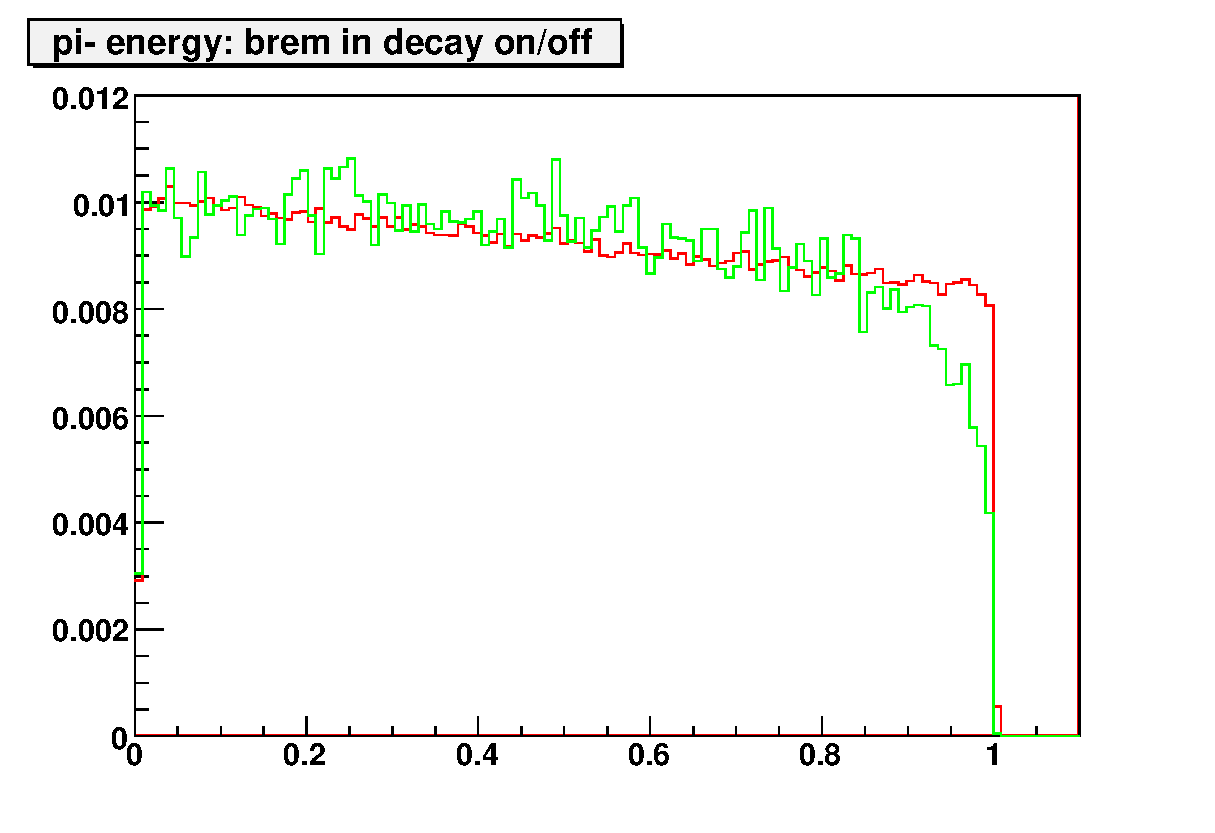
\includegraphics[scale=0.35]{bremdec.eps}
}
\subfigure[bremsstrahlung from $Z$, $\tau^+ $ and $\tau^- $ decays]{
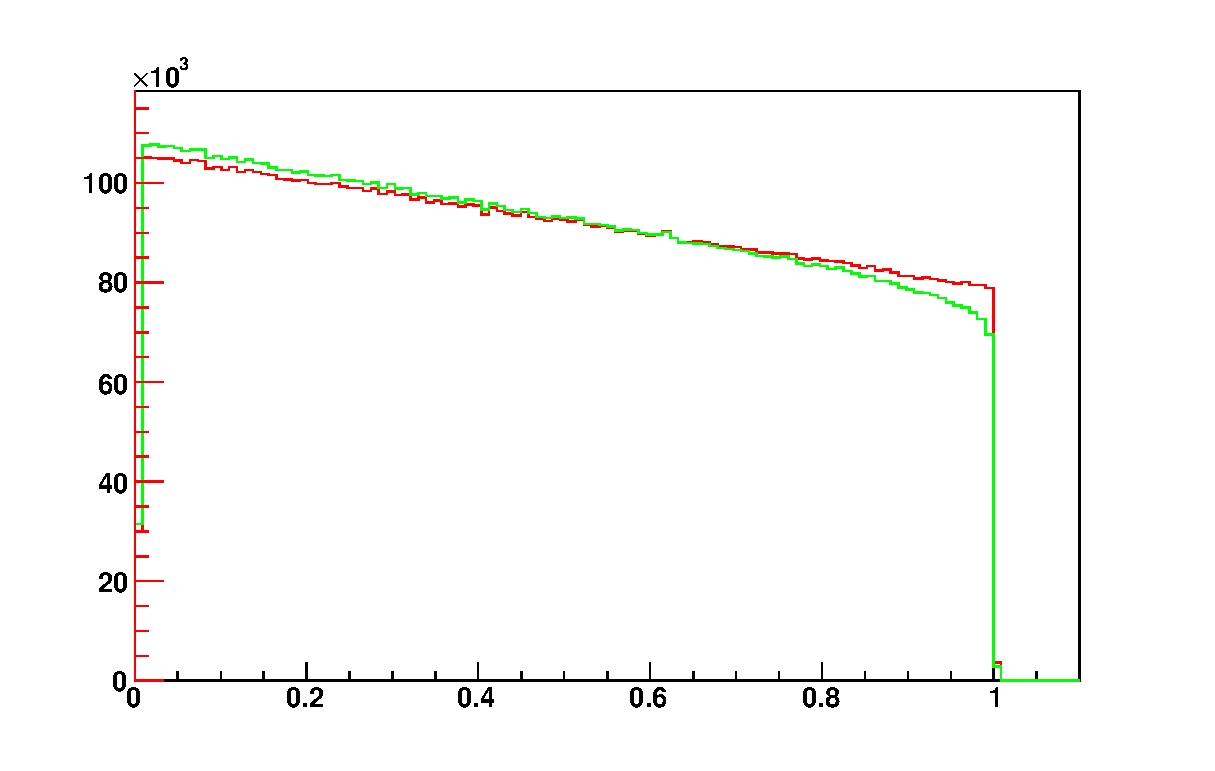
\includegraphics[scale=0.35]{bremall.eps}
}
\caption{ Bremsstrahlung effect for longitudinal spin observable
for cascade decay $Z \to \tau^+ \tau^-$, $\tau^+ \to \pi^+ \nu$,  $\tau^\pm \to \pi^\pm\nu$:
$\pi^+$ energy spectrum in Z rest-frame  is shown. Red line is for 
bremsstrahlung switched off
bremsstrahlung off, green, when its effect is included. 
For left hand side plot,  only  bremsstrahlung in  $\tau^+ $ decay is included.
On right hand side bremsstrahlung from $Z$ and  $\tau^-$ decays are
 also taken into account.
These plots has been created using custom {\tt UserTreeAnalysis} of {\tt MC-TESTER}.
They can be recreated by  test located in {\tt examples/testing/Ztautau} directory, see  {\tt examples/testing/README-plots} for technical details. Results are 
consistent with Fig.~5 of ref.\cite{Eberhard:1989ve}.
\label{fig:KKMC}
}
\end{figure}
\begin{figure}[h!]
\centering
\subfigure[selection C]{
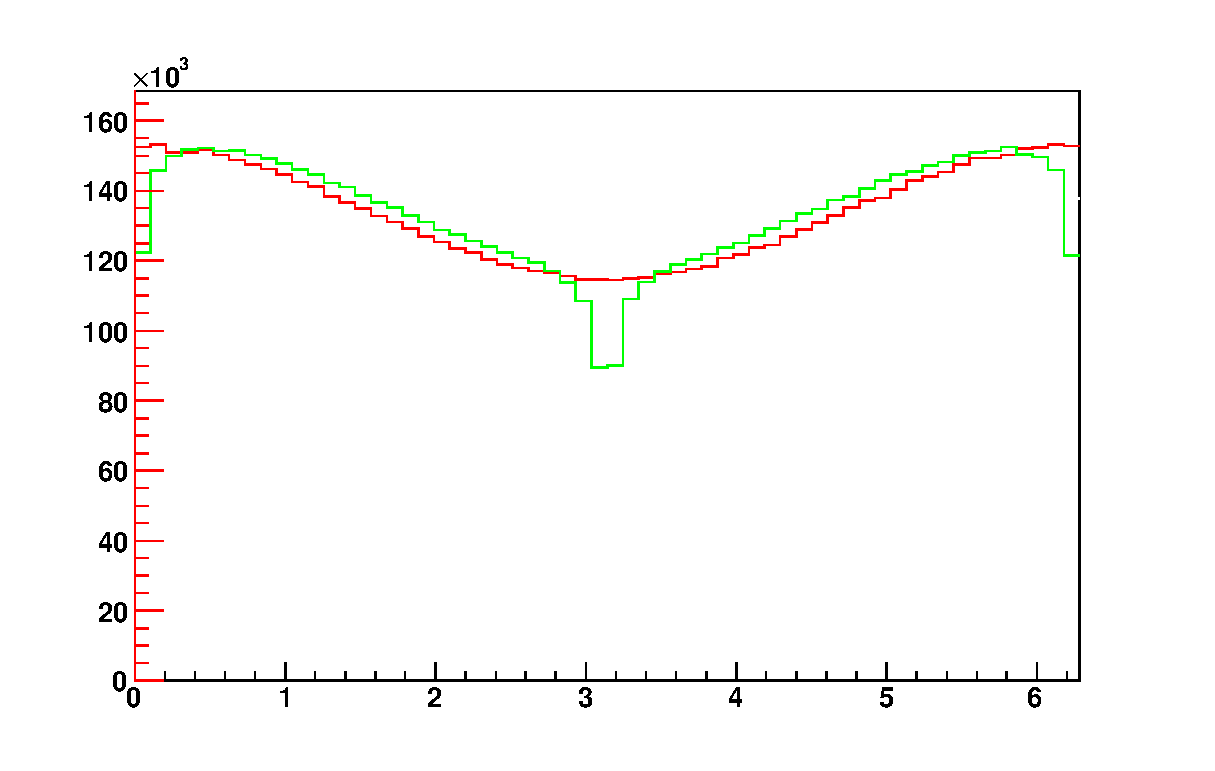
\includegraphics[scale=0.35]{coplanarity-angle-C-photon-over-1-GeV.eps}
}
\subfigure[selection D]{
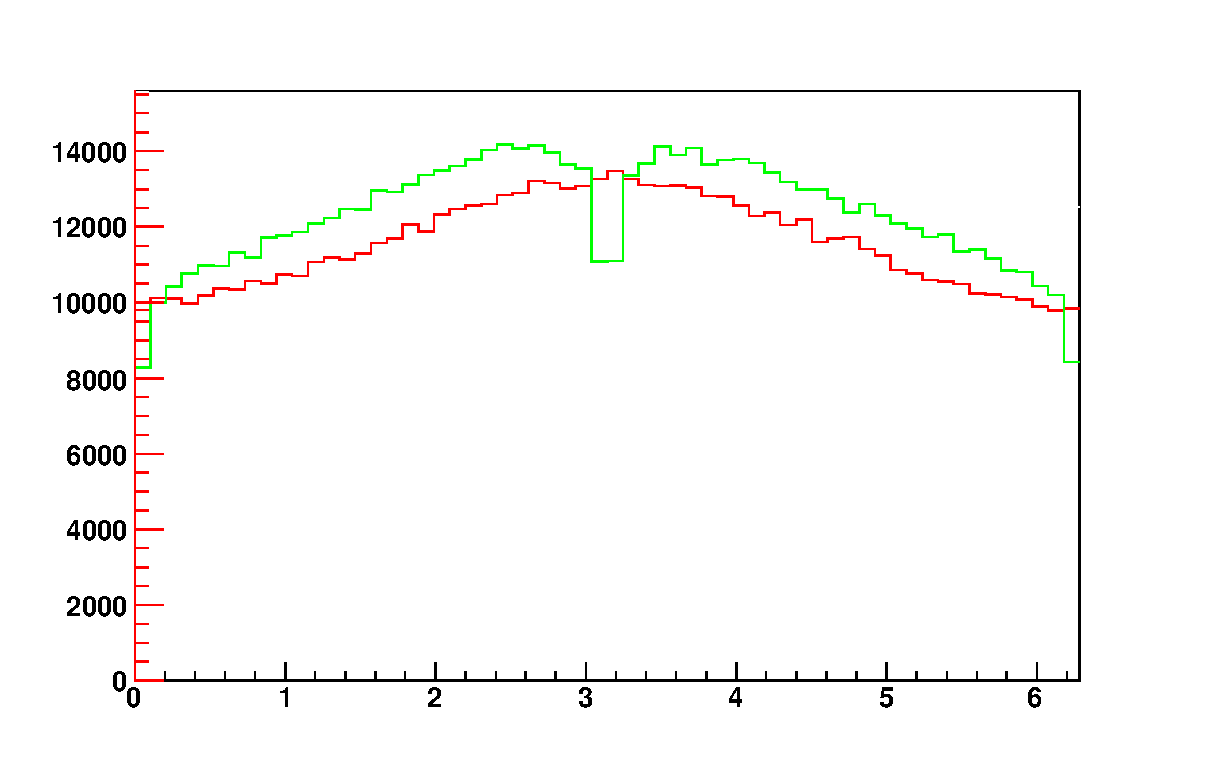
\includegraphics[scale=0.35]{coplanarity-angle-D-photon-over-1-GeV.eps}
}
\caption{Bremsstrahlung effects for transverse spin observable:
In this plot acoplanarity distribution between $\pi^+\rho^+$ and 
$\pi^-\rho^-$ planes in the rest frame of the $\rho+ \rho^-$ pair
for the decay
chain  $H\to \tau^+\tau^-$, $\tau^\pm \to \rho^\pm \nu_\tau$, 
$\rho^\pm \to \pi^\pm \pi^0$, when {\tt PHOTOS} is generating bremsstrahlung is given.
The plots for scalar higgs are given
Red line is for no bremsstrahlung for the green one,
only events where photons of energy larger than 1 GeV in $H$ rest frame are taken.
Note by comparison with fig from ref~\cite{tauolaC++} that kinematical effect
of hard photons are limited to depletion/increase of content of bins for acoplanarity angle close to $0$, $\pi$ and $2\pi$. For definition of selections C and D see.~\cite{Bower:2002zx}.
These plots has been created using custom {\tt UserTreeAnalysis} of {\tt MC-TESTER}.
They can be recreated by performing the test located in {\tt examples/testing/Htautau} directory, see  {\tt examples/testing/README-plots} for technical details.
\label{fig:acoplanarity}
}
\end{figure}

In ref \cite{Adam:2008ge} discussion of systematic errors for measurements of Z cross 
section at LHC is presented. One of the technical tests for the obtained 
distribution is fig 1b of that paper. In our fig \ref{fig:lineshape} we have 
reproduced that plot using {\tt PYTHIA 8.1} and {\tt PHOTOS}. Qualitatively the effect
of FSR QWD bremsstrahlung is in the two cases quite similar. Discussion
of complete electroweak corrections as shown in fig 1a of  \cite{Adam:2008ge}
is not the purpose of our document. Let us point however that electroweak 
non-QED corrections can be installed into {\tt PYTHIA 8.1} {\tt PHOTOS} simulation with 
the help of {\tt TAUOLA} interface \cite{Davidson:2010rw}

let us present LHC oriented plot of Bare electron pair from $Z$ ($W$) decay 
at LHC 
with and without {\tt PHOTOS}. It is similar to plots shown for Horace or Winhac. 
One should bear in mind that this is technical and of little physics direct 
application.
\begin{figure}[h!]
\centering
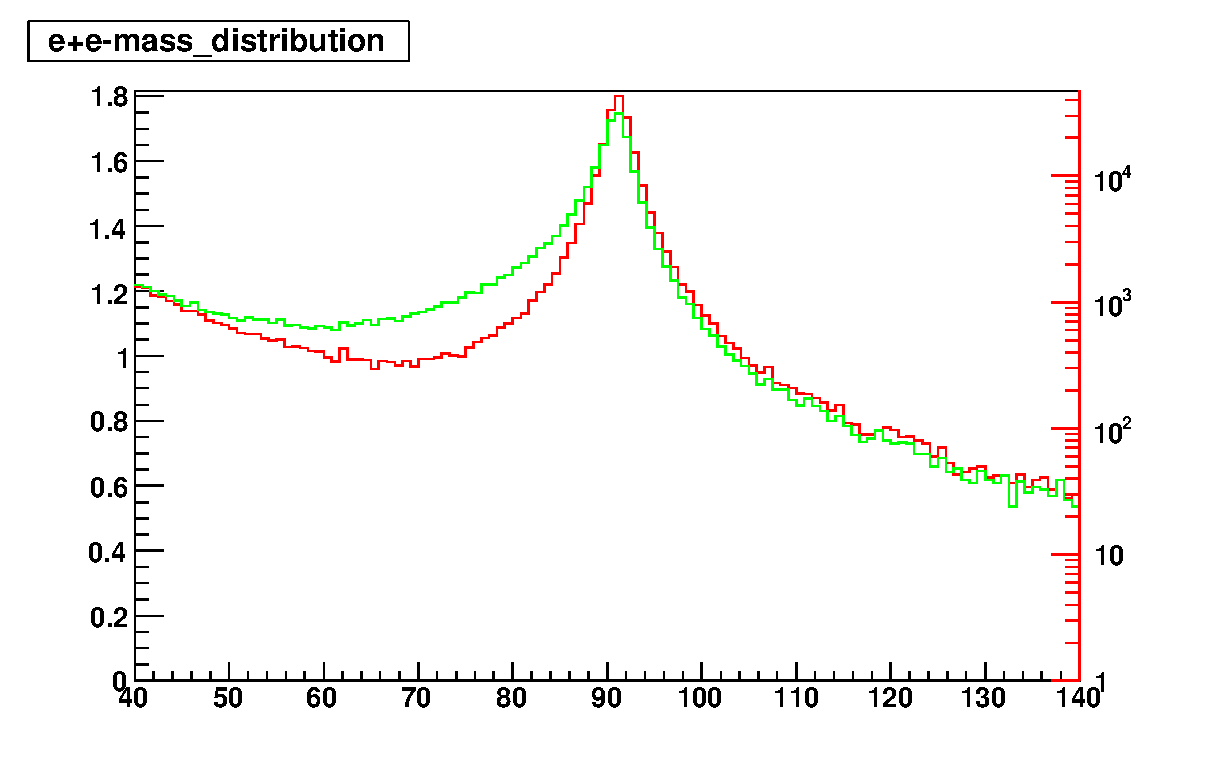
\includegraphics[scale=0.85]{lineshape.eps}
\caption{Distribution of bare $e^+e^-$ invariant mass. Green line represent results when final state 
bremsstrahlung is generated (with the help of {\tt PHOTOS} Monte Calro). For red line FSR 
bremsstrahlung is absent. Event sample is generated with the help of {\tt PYTHIA 8.1}.
Simulation of pp collision at 14 TeV Center of Mass system energy is performed.
$Z/\gamma$ mediated hard process is used.
These plots has been created using custom {\tt UserTreeAnalysis} of {\tt MC-TESTER}.
They can be recreated by performing the test located in {\tt examples/testing/Zee} directory, see  {\tt examples/testing/README-plots} for technical details.
\label{fig:lineshape}
}
\end{figure}

We have checked also that {\tt PHOTOS} works for the $t \bar t$ as well.
For that purpose we have produced the  $t \bar t$ pairs in $pp$ collision at 
14 TeV center of mass energy. We have produced rates for configurations with 0,1 and 
at least two photons of energy above 0.001 of  $t \bar t$ pair mass
(energies are calculated in  hard scattering frame)
results are as in the following Table which is constructed from  
$gg \to t \bar t$ events only:


\vspace{0.3cm} 
\begin{center}
{ \begin{tabular}{|c|c |} 
\hline 
Final state &  Branching Ratio  $\pm$ Rough Errors \\  
\hline 
\hline 
{$ \widetilde{t} t \; \;\; \;$}  &  {99.6118 $\pm$  0.0998\%}  \\ 
\hline 
%\hline 
 {$  \widetilde{t} t \gamma \;\;$} &   { 0.3874 $\pm$  0.0062\%}   \\ 
\hline 
%\hline 
{$  \widetilde{t} t \gamma \gamma$}  &  { 0.0008 $\pm$  0.0003 \%}  \\ 
\hline 
\end{tabular} 
}  
\end{center} 
10 Mevts were generated and slightly modified {\tt LC-analysis} of Ref.~\cite{Golonka:2002rz}
was used for calculation of event rates; no beam was added to list of 
final state particles. Root files for 
differential distributions are 
collected in directory {\tt exaples/testing/ttbar}. 

Let us now turn to example of the test for two photon final state configuration.
We compare KKMC \cite{kkcpc:1999} with exponentiation and second order matrix element 
second order and restricted to first order only, finally results of {\tt PHOTOS} - exponentiation activated. As one can see from the Table. Rates for configurations 
where zero one or at least two photons of energy above 1 GeV are up to two
permille the same for the three cases and $Z\to \mu^+\mu^-$ decay. 

{\centering \begin{tabular}{|c|c|c|c|} 
\hline 
Decay channel &\multicolumn{3}{|c|}{ Branching Ratio $\pm$ Rough Errors}  (100 Mevts samples)\\ 
      & {KKMC CEEX2} & {KKMC CEEX1} & {\tt PHOTOS} exp.\\ 
\hline 
\hline 
 {$Z^{0} \rightarrow \mu^{+} \mu^{-} $} & {83.9190 $\pm$  0.0092\%} &{  83.7841 $\pm$  0.0092\%} & 83.8470 $\pm$ 0.0092 \%\\ 
\hline 
\hline 
 {$Z^{0} \rightarrow \gamma \mu^{+} \mu^{-} $} & {14.8152 $\pm$  0.0038\%} &{  14.8792 $\pm$  0.0039\%} & 14.8589$\pm$ 0.0039\% \\ 
\hline 
\hline 
{$Z^{0} \rightarrow \gamma \gamma \mu^{+} \mu^{-} $} & { 1.2658 $\pm$  0.0011\%} &{   1.3367 $\pm$  0.0012\%} & 1.2940 $\pm$ 0.0011\%\\ 
\hline 
\end{tabular}\par} 
This is not the case for differential distributions, see Fig.~\ref{fig:gamgam}. For example spectrum of 
the two gamma mass is quite different between first and second order 
exponentiation result. This is of potential interest for simulations aiming at 
background for $H \to \gamma \gamma$. In contrary, difference between results from {\tt PHOTOS} and CEEX2 are much smaller. {\tt PHOTOS} exploits first order matrix element 
in a better way than exponentiation. As consequence it reproduce terms resulting in second order leading logarithms. This observation is important not only for 
the particular case of $Z$ decay but for the general case of double bremsstrahlung in any decay as well. That is why it was worth mentioning here.


\begin{figure}[h!]
\centering
\subfigure[CEEX2: red; CEEX1: green]{
\includegraphics[scale=0.35]{{M1@0001.eps}}
}
\subfigure[ CEEX2: red; PHOTOS: green]{
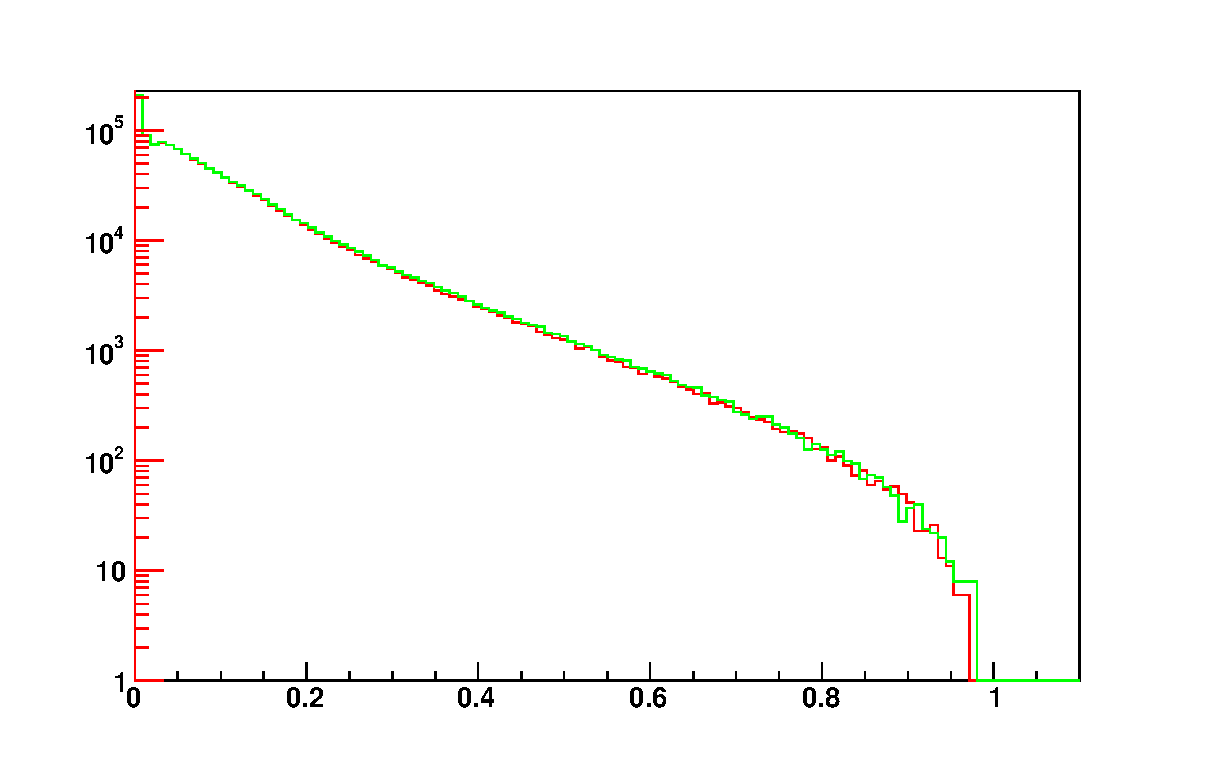
\includegraphics[scale=0.35]{b-M1@0001.eps}
}
\caption{ Spectrum of the $\gamma \gamma$ invariant mass in $Z \to \mu^+\mu^-$
decay. Events with two hard photons, both of energy above 1 GeV in $Z$ rest 
frame are taken. Comparison CEEX2 CEEX1 left hand side plot, and CEEX2 {\tt PHOTOS}
right hand plot. Prediction from {\tt PHOTOS} is clearly superior for applications aiming at
simulation of Higgs boson backgrounds. In case of solutions based on YFS 
exponentiation second order matrix element must be taken into account. Plot b was obtained
from our {\tt examples/testing/Zmumu } after adaptation of center of mass energy 
(91.17 GeV) and test
energy threshold (1 GeV). Samples of 100 Mevts are used. 
See  {\tt examples/testing/README-plots} for technical details, reference 
{\tt mc-tester.root} files for KKMC CEEX samples are however created outside of the distribution.
  \label{fig:gamgam}
}
\end{figure}


Numerical results collected here, provide part of the program benchmarks. 
They are however of  some physics interest as well.
 Photos provides only one step for simulation chain. That is 
bremsstrahlung in decays or final state bremsstrahlung. One can ask 
a question if such specialized unit is of interest and if it is not better 
to provide the complete chain as single simulation package. Obviously this will
depend on particular needs. Theoretically final state QED corrections are 
resonably well separated from remaining genuine electroweak corrections and 
in particular initial state QED bremsstrahlung for quarks if for example 
Drell Yan process at LHC is considered. Such separation may look as unecessary 
complications. However one should bear in mind that final state bremsstrahlund 
need to be disentangled from detector acceptance dependencies and is of not 
interest in itself. If one want to measure propertiex of weak bosons then it 
is natural to cobine their propagators defining their properties together with 
genuine electroweak corrections. Such solution is now available if together 
with PHOTOS interface of electroweak corrections as in TAUOLA Interface is 
provided. 
Finally sizable initial state QED corrections are usually embodied in  units 
simulating parton showers. This may need some experimental analysis as well. 
Recently experimental data of LEP1 time are revisited \cite{Abdallah:2010tk} 
by DELPHI collaboration. Tension of data with theoretical description is 
mentioned. This may mean that description of initial state QED bremsstrahlung 
at LHC will need to be reinvestigated with the help of LHC data as well.





\section{Summary and outlook}
We have presented new version  of {\tt PHOTOS} Monte Carlo. The part operating on 
event record is rewritten now to C++ and uses for input the HepMC event record 
format. Physics performance of the algorithm is the same  as this of 
{\tt FORTRAN/HEPEVT} version. Steps toward future improvements are prepared. 
Whenever algorithm for modification of elementary decay is involved its 
kinematical configuration is boosted to decay particle rest frame, which 
z axis is oriented along momentum of the first decaying particle (object) 
rest frame. Thanks to this extension  installation of process dependent 
kernels featuring complete first order matrix element will be possible.
If of numerical interest appropriate corrections explained in 
refs.~\cite{Golonka:2006tw,Nanava:2006vv,Nanava:2009vg}  will have necessary input prepared.
At present parts of the algorithm are left in {\tt FORTRAN}. This part of the code 
will be rather easy to change to C++. No obstacles are expected. However as this part of the code does not require any special data structures expected gains
except code homogenity are rather minimal.  

\vskip 2 mm

\centerline{\large\bf Acknowledgements}


Useful discussions with P. Golonka during the early stage of project development and discussions 
with members of the ATLAS and CMS collaborations, and the LCG group are acknowledged.
We are specially indebted to the pilot users of the interface, in particular to:
...

Partial support of Polish-French collaboration
no. 06-124 within IN2P3 through LAPP Annecy and 
during final completion of this work is
also acknowledged.

\newpage

\bibliography{Photos_interface_design}{}
\bibliographystyle{plain}






%------------------------------------------------------------------------------
\newpage
\appendix

\section{Appendix: Interface to {\tt PHOTOS FORTRAN}}
\label{Interface to PHOTOS}

This section is addressed to developers of the interface, 
and special users interested in advanced options of {\tt PHOTOS FORTRAN}.
For this purpose we describe the common blocks and routines which allow
communication between {\tt PHOTOS} and {\tt PHOTOS} C++ Interface.

\subsection{Common Blocks}

In the following let us list common blocks of {\tt PHOTOS} which are accessed
from C++.

\begin{description}
\item[PHOCOP] Coupling constant and related parameters.
    \begin{description}
	\item[ALPHA]  \textit{double}  coupling constant $\alpha_{QED}$.
	\item[XPHCUT] \textit{double} minimal energy (in units of decaying particle mass) for photons to be explicitly generated.
    \end{description}
\end{description}

\begin{description}
\item[PHOKEY] keys and parameters controlling algorithm options.
    \begin{description}
	\item[FSEC]   \textit{double} internal variable for algorithm options, default is FSEC-1..
	\item[FINT]   \textit{double} Maximum interference weight.
	\item[EXPEPS] \textit{double} Technical parameter, blocks crude level high photon multiplicity from configurations less probable than EXPEPS, default is $10^{-4}$.
	\item[INTERF] \textit{bool} Key for interference, matrix element weight.
	\item[ISEC]   \textit{bool} switch for double bremsstrahlung generation.
	\item[ITRE]   \textit{bool} switch for bremsstrahlung generation up to multiplicity 4.
	\item[IEXP]   \textit{bool} switch for exponentiation mode.
	\item[IFTOP]  \textit{bool} switch for photon emission in top pair production in quark (gluon) pair annihilation.
    \end{description}
\end{description}

\begin{description}
\item[PHSEED] common block for a copy of Marsaglia and Zaman random number generator used in {\tt FORTRAN} part of {\tt PHOTOS}.
    \begin{description}
	\item[ISEED[ 2]]  \textit{int} seed values, default is  ISEED[ 1]=1802, ISEED[ 2]=9373
	\item[I97]        \textit{int} internal variable of the random number generator.
	\item[J97]        \textit{int} internal variable of the random number generator.
	\item[URAN[ 97]]  \textit{double} internal variable of the random number generator.
	\item[CRAN]       \textit{double} internal variable of the random number generator.
	\item[CDRAN]      \textit{double} internal variable of the random number generator.
	\item[CMRAN]      \textit{double} internal variable of the random number generator.
    \end{description}
\end{description}

\begin{description}
\item[PHLUPY] Debug messages handling
    \begin{description}
    \item[IPOIN]  \textit{int} Messages above this value will not be displayed
	\item[IPOINM] \textit{int} Messages below this value will not be displayed
    \end{description}
\end{description}

\begin{description}
\item[PH\_PHOQED] Supplement for PH\_HEPEVT event record to block emission 
from some particles.
    \begin{description}
    \item[QEDRAD[ 10000]]  \textit{bool} flag enabling {\tt FORTRAN} user
    to block emission from particles stored in PH\_HEPEVT. Not used in 
     our interface.
    \end{description}
\end{description}

\subsection{Routines}

In the following let us list routines which are called from the interface.

\begin{description}
\item[PHOINI] initialize generator, use as input content of common blocks. \\
  Return type: \textit{void} \\
  Parameters: none
\end{description}

\begin{description}
\item[PHODMP] Prints out the content of HEPEVT. \\
  Return type: \textit{void} \\
  Parameters: none
\end{description}

\begin{description}
\item[PHOTOS\_MAKE] {\tt FORTRAN} part of interface. \\
  Return type: \textit{void} \\
  Parameters:
  \begin{enumerate}
    \item \textit {int id} ID of particle from which {\tt PHOTOS} starts processing. In C++ case importance of this parameter is limited as only one branch is in HEPEVT at a time.
  \end{enumerate}
\end{description}

\begin{description}
\item[PHCORK] Initializes Kinematic Corrections. \\
  Return type: \textit{void} \\
  Parameters:
  \begin{enumerate}
    \item \textit {int modcor} Type of correction. See {\tt FORTRAN} documentation for details.
  \end{enumerate}
\end{description}

\section{Appendix: User Guide}
\label{sec:User Guide}

\subsection{Installation}
\label{sec:Installation}
The main interface library requires that {\tt HepMC} \cite{Dobbs:2001ck} (version 2.04 or later)  has been installed
and its location has been provided during the configuration step. This is sufficient to compile the interface and to run the simple, standalone example.

However, in order to run more advanced examples located in the {\tt /examples} directory, it is required to install also:

\begin{itemize}
  \item {\tt ROOT} \cite{root-install-www} version 5.18 or later
  \item {\tt PYTHIA 8.1} \cite{Sjostrand:2007gs} or later. {\tt PYTHIA 8.1} must be compiled with {\tt HepMC} 2.xx
        so that the {\tt PYTHIA} library {\tt hepmcinterface} exists.
  \item {\tt MC-TESTER} \cite{Golonka:2002rz,Davidson:2008ma} version 1.24 or later.
        Do not forget to type {\tt make libHepMCEvent} after compilation of {\tt MC-TESTER} is done.
  \item {\tt TAUOLA} \cite{Davidson:2010rw} version 1.02 or later.
\end{itemize}

In order to compile the {\tt PHOTOS} C++ Interface:
\begin{itemize}
 \item Execute {\tt ./configure} with the additional command line options:
   \subitem {\tt --with-HepMC=$<$path$>$} provides the path to the {\tt HepMC} installation directory. One can also set the {\tt HEPMCLOCATION} variable instead of using this directive. This path is required for the interface to compile.
   \subitem {\tt --prefix=$<$path$>$} provides the installation path. The {\tt include} and {\tt lib} directories will be copied there if {\tt make install} is executed later. If none has been provided, the default directory for installation is {\tt /usr/local}.
 \item Execute {\tt make}
 \item Optionally, execute {\tt make install} to copy files to the directory provided during configuration.
\end{itemize}

The {\tt PHOTOS} C++ interface will be compiled and the {\tt /lib} and {\tt /include} directories will contain the appropriate libraries and include files.

In order to compile the examples, compile {\tt PHOTOS} C++ interface and enter the {\tt /examples} directory and:
\begin{itemize}
  \item Execute {\tt ./configure} to determine which examples can be compiled.
        Additional paths can be provided as command line options:
   \subitem {\tt --with-Pythia8=$<$path$>$} provides the path to the {\tt Pythia8} installation
            directory. One can set the {\tt PYTHIALOCATION} variable instead of using this directive.
            This path is required for all examples and tests.
   \subitem {\tt --with-MC-Tester=$<$path$>$} provides the path to the {\tt MC-TESTER} installation
            directory (the {\tt libHepMCEvent} must be compiled as well, see \cite{Davidson:2008ma}
			for more details). One can set the {\tt MCTESTERLOCATION} variable instead of using this
			directive. This path is required for all additional examples and tests.  This option
			implies that {\tt ROOT} has already been installed (since it is required by {\tt MC-TESTER}).
			The {\tt ROOT} directory {\tt bin} should be listed in variable {\tt PATH} and {\tt ROOT}
			libraries in {\tt LD\_LIBRARY\_PATH}.
   \subitem {\tt --with-Tauola=$<$path$>$} provides the path to the {\tt TAUOLA} installation directory.
            One can set the {\tt TAUOLALOCATION} variable instead of using this directive.
			This path is required for additional examples only.
  \item execute {\tt make}
\end{itemize}

If neither {\tt Pythia8} nor {\tt MC-TESTER} are present, only the simple example will be provided. The {\tt /examples} directory will contain the compiled example files.

\subsection{Elementary Tests}
\label{sect:elem}
The most basic test which should be performed is verification that the interface is installed correctly, that all
photons are indeed added by the program and that energy momentum conservation is preserved.

Once correct execution of the basic program steps have been confirmed,
step one of the program installation tests  is completed\footnote{
We have  performed such  tests for all choices of the {\tt HepMC} event record obtained 
from  {\tt PYTHIA 8.1} processes and 
listed later in the paper. Further  options for initializations 
(parton shower hadronization or QED bremsstrahlung on/off etc.) were studied.
This installation step  was a necessary one of program development as well.}.

In principle, these tests have to be performed for any new hard 
process and after any new installation. This is to ensure that 
information is passed from the event record to the interface 
correctly and that physics information is filled into {\tt HepMC} 
in expected manner. Misinterpretation of the event record content may result in 
faulty generation by {\tt PHOTOS}.


\subsection{Executing Examples}

Once elementary tests are completed one can turn to the more advanced ones.
The purpose is not only to validate the installation but to demonstrate how the
interface can be used.

The examples can be run by executing the appropriate {\tt .exe} file in the {\tt /examples} directory.
In order to run some more specific tests for the following processes:
$H \rightarrow \tau^+ \tau^-$, $ e^+ e^- \rightarrow t \bar t$,
$W \rightarrow e \nu_e$, $W \rightarrow \mu \nu_\mu$,
$Z \rightarrow e^+ e^-$ or $Z \rightarrow \mu \mu$,
the main programs residing in subdirectories of the same name placed in the
{\tt /examples/testing} directory should be executed.
In all cases the following actions have to be performed:

\begin{itemize}
  \item Compile {\tt PHOTOS } C++ Interface as well as the examples. 
 \item  Check that the appropriate system variables are set: normally set by the script \\
{\tt /configure.paths.sh} (the configuration step mentions this script).
  \item Enter the {\tt /examples/testing} directory. Modify test.inc if needed.
  \item enter the chosen directory and execute {\tt make}.
\end{itemize}

The appropriate .root files as well as .pdf files generated by {\tt MC-TESTER}
will be created inside the chosen directory. One can execute 'make clobber' to
clean the directory. One can also execute 'make' inside the {\tt /examples/testing}
directory to run all available tests one after another. New source
code changes can easily be validated in this way.
Tests are run using {\tt examples/photos\_pythia\_example.exe} 
and booklets will be produced with comparisons to the benchmark files.

A set of benchmark {\tt MC-TESTER} root files are packed with the interface
distribution in the subdirectories of {\tt examples/testing/}. They can be used
as examples to start new work or simply to construct comparison
plots to validate new versions or new installations of {\tt PHOTOS} interface.

In Appendix \ref{sec:User Configuration} possible modifications to the  
examples settings are discussed. This may be interesting as an initial step for users 
physics studies.  Numerical results of some of these tests are collected in Section \ref{sec:results}
and can be thus reproduced by the user.

\subsection{How to tun {\tt PHOTOS} with other generators}
If user is building large simulation system he may want to avoid our 
infrastructure and load only libraries. For that purpose our stand-alone 
example is good starting point.

In order to link the libraries to the user's project, both the static libraries and shared objects are
constructed. To use {\tt PHOTOS} interface in an external project additional 
compilation directives are required. For the static libraries:
\begin{itemize}
  \item add {\tt -I<PhotosLocation>/include } at the compilation step,
  \item add {\tt <PhotosLocation>/lib/libPhotosCxxInterface.a } and\\
        {\tt <PhotosLocation>/lib/libPhotosFortran.a } at the linking step.
\end{itemize}
For the shared objects:
\begin{itemize}
  \item add {\tt -I<PhotosLocation>/include } at the compilation step,
  \item add {\tt -L<PhotosLocation>/lib } along with {\tt -lPhotosCxxInterface } at the linking step.
  \item  {\tt PHOTOS} libraries must be provided for the executable; eg. with the help of  {\tt LD\_LIBRARY\_PATH }.
\end{itemize}
The {\tt <PhotosLocation>} denotes the path to {\tt PHOTOS} installation directory.
In most cases it should be enough to include {\tt Photos.h} and {\tt PhotosEvent.h}
within user program and use {\tt PHOTOS} class for configuration and {\tt PhotosEvent}
for event processing.

\section{Appendix: User Configuration}
\label{sec:User Configuration}

\subsection{Suppress Bremsstrahlung}
\label{section:suppress}

In general, {\tt PHOTOS} will attempt generation of bremsstrahlung in every 
branching point. This is of course not always appropriate.
Already inside {\tt FORTRAN} bremsstrahlung will be prevented for vertices featuring gluons or quarks.
The only exception is top quark. This is not enough. By default we eliminate 
generation for vertices like $l^\pm \to l^\pm \gamma$ due to self-decay.
We can not request that all incoming and/or outgoing 
lines are on mass shell, because it is not the case in cascades featuring 
intermediate states of sizable width. If some parton shower feature
vertex  $l^\pm \to l^\pm \gamma$ of virtuality of incoming $l^\pm$ 
matching the invariant mass of the outgoing pair then {\tt PHOTOS} will act
obviously introducing error. This can be prevented if generation from vertices
with one of the decay products flavour matching flavour of incoming 
one is forbidden. Not always such exclusion should take place. For example
in cascade decays vertex $\rho \to \rho \pi$ may require algorithm to be 
active. Methods to enable special cases of previously prevented classes, or to
prevent generation in special branches have been introduced and presented in the next section.
This may be necessary for combination of consecutive branchings. For example if bremsstrahlung
in leptonic $\tau$ decay is generated by programs prior to {\tt PHOTOS}, and decay is coded in HepMC as cascade $\tau^\pm \to W^\pm \nu$, $W^\pm \nu \to l^\pm \nu$
{\tt PHOTOS} must be prevented to act if such vertices are stored consecutively.
One can think also of special cases of the following type:
if vertex $q \bar q \to l^\pm l^\mp$ is found then it should not be ignored
but passed for generation as $q \bar q \to Z \to l^\pm l^\mp$ where intermediate Z is created internally for {\tt PHOTOS}. \\
\\
For user convenience the following configuration methods are provided:
\begin{itemize}
 \item {\tt Photos::suppressBremForDecay(daughterCount, motherID, d1ID, d2ID, ...)} \hfill \\
       The basic use of channel suppression, by providing number of daughters,
	   PDGID of the mother and the list of PDGIDs of daughters.
	   There's no upper limit of the number of daughters.
	   If a decay with the matching pattern is found, {\tt PHOTOS} will skip the corresponding decay.
 \item {\tt Photos::suppressBrem(0, motherID)} \hfill \\
       When only the PDGID of the mother is provided, {\tt PHOTOS} will skip all decay channels
	   of this particle. Note, that you still have to provide the number of daughters,
	   which in this case is zero.
 \item {\tt Photos::suppressBremForBranch(daughterCount, motherID, d1ID, d2ID, ...)} \hfill \\
       {\tt Photos::suppressBremForBranch(0, motherID)} \hfill \\
       The usage is similar to the above function. The difference is,
	   that if {\tt PHOTOS} finds the matching decay channel, it will skip not only the corresponding channel,
	   but also all consecutive decays of it's daughters, making {\tt PHOTOS} skip the whole branch
	   of decays instead of just one listed decay.
 \item {\tt Photos::suppressAll() }
       All branchings will be suppressed except those that are forced using routines
	   described in the next section.
 \item \textbf{Example:} \hfill \\
{\tt Photos::suppressBremForDecay(4, 15, 16, -211, 300, -400); } \\
{\tt Photos::suppressBremForDecay(2, -15, -16, 211); } \\
{\tt Photos::suppressBremForDecay(0, 211); } \\
\emph{If the decays {\tt 15 => 16, -211, 300, -400} or {\tt -15 => -16, 211} are found, they will be skipped by {\tt PHOTOS}. In addition, all decays of particle {\tt 211} will also be skipped. Note, that the minimum number of parameters that must be provided is two - the number of daughters (which can be zero) and the mother PDGID.} \\ \\
{\tt Photos::suppressBremForBranch(2, 15, 16, -211); } \\
\emph{When a decay {\tt 15 => 16, -211 } is found, it will be skipped by {\tt PHOTOS} along with the decays of particle 16, -211 and all their daughters. In the end, the whole decay tree starting with {\tt 15 => 16, -211} will be skipped.}
\end{itemize}

\subsection{Force {\tt PHOTOS} processing }
\label{section:force}

For example, suppress all, then turn on any appropriate process.

Forcing processing using methods below has higher priority than suppressing described
in previous section, therefore even if both forcing and suppressing of the same
branch or decay is done (no matter in which order), the processing will not be
suppressed.

\begin{itemize}

 \item {\tt Photos::forceBremForDecay(daughterCount, motherID, d1ID, d2ID, ...)} \hfill \\
       {\tt Photos::forceBremForDecay(0, motherID)} \hfill \\
       The usage of this routine is similar to {\tt Photos::suppressBremForDecay(...)}
	   described in previous section. If a decay with the matching pattern is found,
	   {\tt PHOTOS} will be forced to process corresponding decay, even if it was suppressed
	   by any of the methods mentioned in previous section.
 \item {\tt Photos::forceBremForBranch(daughterCount, motherID, d1ID, d2ID, ...)} \hfill \\
       {\tt Photos::forceBremForBranch(0, motherID)} \hfill \\
       The usage is similar to the above function. The difference is,
	   that if {\tt PHOTOS} finds the matching decay channel, it will force not only the corresponding channel,
	   but also all consecutive decays of it's daughters, making {\tt PHOTOS} process the whole branch
	   of decays instead of just one listed decay.
 \item \textbf{Example:} \hfill \\
{\tt Photos::suppressAll(); } \\
{\tt Photos::forceBremForDecay(4, 15, 16, -211, 300, -400); } \\
{\tt Photos::forceBremForDecay(2, -15, -16, 211); } \\
{\tt Photos::forceBremForBranch(0, 211); } \\
\emph{Since suppressing of all processing is used, only the listed decays will be processed, that is
{\tt 15 => 16, -211, 300, -400} or {\tt -15 => -16, 211} and all decays of particle {\tt 211} and
all its daughters.}
\end{itemize}

\subsection{Use of {\tt processParticle} and {\tt processBranch} methods}
\label{PHOTOSgun}

In Section~\ref{sect:Outline} an algorithm to process whole event record is explained.
For that purpose {\tt process()} method is provided.
To process a single branch in a way independent of the
event record content another, simple method is provided.

\begin{itemize}
  \item {\tt Photos::processParticle(PhotosParticle *p) } \hfill \\
		The main routine for processing a single particle. When a pointer to particle
		is provided, from this particle a branch containing its mothers and daughters
		will be created and processed by {\tt PHOTOS}.
  \item {\tt Photos::processBranch(PhotosParticle *p) } \hfill \\
 		When a pointer to particle is provided, {\tt PHOTOS} will process the whole decay
		tree starting from the particle	provided as pointer.
\end{itemize}

An example {\tt single\_photos\_gun\_example.c} is provided in the directory {\tt /examples}
showing how this functionality can be used to process a decay of selected particles.
The $Z0 \rightarrow \tau^+ \tau^-$ decays are generated and the event record is traversed
searching for the first $\tau^-$ particle found in event record.
Instead of processing the whole event, only the decay of $\tau^-$ is processed by {\tt PHOTOS}.


\subsection{Logging and Debugging}
\label{App:Logging}
This section describes the basic functionality of the logging and debugging tool.
For details on its content we address the reader to comments in the {\tt /src/utilities/Log.h} header file.

Let us present however some general scheme of the tool functioning.
{\tt PHOTOS} interface allows filtering out some amount of data displayed during the program run
and provides a basic tool for memory leak tracking. The following functions
can be used from within the user program after including the {\tt Log.h} file:
\begin{itemize}
  \item {\tt Log::Summary() } - Displays a summary of all messages.
  \item {\tt Log::SummaryAtExit() } - Displays the summary at the end of a program run.
  \item {\tt Log::LogInfo(bool flag) } \\
        {\tt Log::LogWarning(bool flag) } \\
        {\tt Log::LogError(bool flag) } \\
        {\tt Log::LogDebug(int s, int e) } \\
        {\tt Log::LogAll(bool flag)} \\
        Turns logging of info, warning, error and debug messages on and off depending
        on the flag being true or false. In the case of debug messages - the range of codes
        to be displayed must be provided. By default, only debug messages
        (from 0 to 65535) are turned off. If the range is negative ($s>e$) the debug messages
        won't be displayed. The last option turns displaying all of the above messages on and off.
  \item {\tt Log::LogPhlupa(int from, int to) } \\
        Turns logging of {\tt FORTRAN} debug messages on and off.
\end{itemize}

Additionally, option {\tt Log::SetWarningLimit(int limit)} is available, allowing
only first {\tt `limit'} warnings to be displayed. The default for {\tt limit} is 100. 
If {\tt limit}=0 is chosen then no limits on warnings display will be set.

The memory leak tracking function allows checking of whether all memory allocated within {\tt PHOTOS Interface}
 is properly released. However, using the debug option significantly increases the amount of time needed for 
each run. Its  use is therefore recommended  for debugging purposes only. In order to use this option
 modify {\tt make.inc} in the main directory by adding the line: \\
\\ {\tt DEBUG = -D"\_LOG\_DEBUG\_MODE\_" } \\ \\
Recompile the interface.
Now, whenever the program is executed a table will be printed at the end of the run,
listing all pointers that were not freed, along with the memory they consumed.
If the interface works correctly without any memory leaks, one should get an empty table.

It is possible to use this tool within the user program, however there are a few limitations.
The debugging macro from "Log.h" can create compilation errors if one compiles
it along with software which has its own memory management system (e.g. {\tt ROOT}).
To make the macro work within a user's program, ensure that {\tt Log.h} is the last header file
included in the main program.
It is enough to  compile the program with the {\tt -D"\_LOG\_DEBUG\_MODE\_" } directive added,
or {\tt \#define \_LOG\_DEBUG\_MODE\_ } placed within the program before include
of the {\tt Log.h} file%
\footnote{Note that {\tt Log.h } does not need to be included within
the user program  for the memory leak tracking tool to be used only for {\tt PHOTOS} interface.
}.

\subsection{Other User Configuration Methods}
\label{subsection:other_methods}

The following auxiliary methods are prepared. They are useful for initialization 
or are introduced for backward compatibility.

\begin{itemize}
  \item {\tt Photos::setSeed(int iseed1, int iseed2)} \\
        Set internal {\tt FORTRAN} RANMAR random generation seed values.
   \item {\tt Photos::maxWtInterference(double interference)} \\
        Set maximum interference weight. The default is 2.
\end{itemize}

\subsection{Creating advanced plots and custom analysis}
\label{App:Plots}

In Section \ref{sec:results}, we've presented results of a non-standard
analysis performed by {\tt MC-Tester}. Figure \ref{fig:lineshape} has been
obtained by using custom {\tt UserTreeAnalysis} located in file {\tt ZeeAnalysis.C}
residing in {\tt examples/testing/Zee} directory. This file serves as an
example of how the custom analysis can be introduced and new plots can be
added to the project with the help of {\tt MC-Tester}.

The basic {\tt MC-Tester} analysis contains methods used by pre-set examples
in {\tt examples/testing} directory to limit the number of soft photons generated
by {\tt PHOTOS}. It's description and usage has already been documented in \cite{Davidson:2008ma}.
The content of {\tt ZeeAnalysis.C} is identical to the default {\tt UserTreeAnalysis}
of {\tt MC-Tester} with the only addition being the simple method to create
previously mentioned plot.

In order to create a $t \bar t$ example that {\tt PHOTOS} is able to process,
two additional routines had to be added to {\tt photos\_pythia\_example.c}.
These routines - {\tt electronToGluon} and {\tt fixForMctester} are necessary
due to the uniqueness of the generated process.

Due to {\tt PYTHIA} generating a large amount of vertices where momentum is not
conserved for all $p p \rightarrow t \bar t$ processes, in order to present this
example we have used a much more stable $e^+ e^- \rightarrow t \bar t$
generation. However, the {\tt FORTRAN} version of {\tt PHOTOS} has not been designed
to work with such process, therefore a quick fix converting the pdg ID of
the incoming particles from electrons to gluons has been introduced.

Additionally, since {\tt MC-Tester} is not designed to analyze processes involving
multiple incoming particles, we've used a simple method similar to previously
used in {\tt FORTRAN} examples {\tt LC\_Analysis} mentioned in \cite{Golonka:2002rz}, Section 6.1. However,
this method proved to be hard to implement with current version of {\tt HepMC}
interface of {\tt MC-Tester}, therefore a special routine had to be added
to add similar modifications to {\tt HepMC} event. This modification transforms
$X Y \rightarrow t \bar t$ process to $100 \rightarrow Y t \bar t$ process,
where the momentum of special particle $100$ is $X + 2*Y$ so that momentum is still
conserved within the vertex. With that modification, {\tt MC-Tester} can be set up
to analyze particle $100$ in order to get a desirable results.

%------------------------------------------------------------------------------
\newpage

\section*{Task List}
In this section we provide a check-list of incomplete tasks.
This could be used as a guide for project planning and is foreseen
to be a working document. 

(prioritized: {\bf 1} - Highest priority. The program should not be
released without this task being completed. {\bf 2} - Medium priority.
It should be clearly documented for developers and users that this task has not
been completed. {\bf 3} - Lowest priority such as a long term goal 
for the project).

\subsection*{Functionality}
\begin{itemize}
  \item[\ding{111}]{\bf 1} - Complete example t tbar
  \item[\ding{111}]{\bf 2} - Remove dead {\tt FORTRAN} code
  \item[\ding{111}]{\bf 2} - Rewrite parts on HEPEVT type data structure
  \item[\ding{111}]{\bf 3} - Move {\tt FORTRAN} remnants to C++
\end{itemize}

\subsection*{Testing}
\begin{itemize}
  \item[\ding{111}]{\bf 1} - Long run root files for tests e+e- and pp
  \item[\ding{111}]{\bf 1} - missing plots for documentation benchmarks
  \item[\ding{111}]{\bf 2} - event record options
  \item[\ding{111}]{\bf 3} - further plots of some interest
\end{itemize}

\subsection*{Usability}
\begin{itemize}
  \item[\ding{111}]{\bf 1} - paper complete
  \item[\ding{111}]{\bf 1} - READMES 
  \item[\ding{111}]{\bf 2} - paper cleaning
  \item[\ding{111}]{\bf 2} - User interaction and resulting fixes
  \item[\ding{111}]{\bf 3} - Doxygen documentation update
\end{itemize}


\end{document}
